\documentclass[11pt]{article}

% ---------- fonts & base ----------
\usepackage[T1]{fontenc}
\usepackage[utf8]{inputenc}
\usepackage{charter}
\usepackage{courier}
\usepackage{microtype}
\usepackage[margin=1.05in,headheight=14pt]{geometry}
\usepackage{graphicx}
\usepackage{xcolor}
\usepackage{tikz}
\usetikzlibrary{arrows.meta,positioning,shapes.misc,calc,fit,backgrounds}
\usepackage{tcolorbox}
\tcbuselibrary{skins,breakable}
\usepackage{booktabs,longtable,array,ragged2e}
\usepackage{enumitem}
\usepackage{titlesec}
\usepackage{fancyhdr}
\usepackage[hidelinks]{hyperref}
\usepackage{setspace}

% ---------- palette ----------
\definecolor{slate}{HTML}{23303E}
\definecolor{honey}{HTML}{A8720E}
\definecolor{honeypale}{HTML}{FBF4E2}
\definecolor{inkgrey}{HTML}{55606C}
\definecolor{palegrey}{HTML}{F2F3F5}

% ---------- headings ----------
\titleformat{\section}{\Large\bfseries\color{slate}}{\thesection}{0.7em}{}
\titleformat{\subsection}{\large\bfseries\color{slate}}{\thesubsection}{0.6em}{}
\titleformat{\subsubsection}{\normalsize\bfseries\color{inkgrey}}{\thesubsubsection}{0.6em}{}
\titlespacing{\section}{0pt}{1.4em}{0.7em}
\titlespacing{\subsection}{0pt}{1.1em}{0.5em}

% ---------- headers ----------
\pagestyle{fancy}
\fancyhf{}
\fancyhead[L]{\small\color{inkgrey}OmegaHive: A Running Hive}
\fancyhead[R]{\small\color{inkgrey}\thepage}
\renewcommand{\headrulewidth}{0.3pt}
\renewcommand{\headrule}{\color{palegrey}\hrule width\headwidth height 0.6pt}

% ---------- excerpt box (Ben's specs) ----------
\newtcolorbox{benquote}[1][]{
  enhanced, breakable,
  colback=honeypale, colframe=honeypale,
  borderline west={2.2pt}{0pt}{honey},
  left=8pt, right=8pt, top=6pt, bottom=6pt,
  boxrule=0pt, arc=1.5pt,
  fontupper=\small,
  #1
}
\newcommand{\benattrib}[1]{\par\smallskip\raggedleft\footnotesize\color{inkgrey}--- #1\par}

% ---------- aside box (worked examples / stories) ----------
\newtcolorbox{casebox}[1][]{
  enhanced, breakable,
  colback=palegrey, colframe=palegrey,
  borderline west={2.2pt}{0pt}{slate},
  left=8pt, right=8pt, top=6pt, bottom=6pt,
  boxrule=0pt, arc=1.5pt,
  fontupper=\small,
  title={}, #1
}

% ---------- misc ----------
\newcommand{\code}[1]{\texttt{\small #1}}
\setlist{itemsep=2pt,topsep=4pt}
\setlength{\parskip}{0.35em}
\setlength{\parindent}{0pt}
\newcolumntype{L}[1]{>{\RaggedRight}p{#1}}

% TikZ shared styles
\tikzset{
  hbox/.style={draw=slate, fill=white, rounded corners=2pt, thick, align=center, font=\small, inner sep=5pt},
  hboxaccent/.style={hbox, draw=honey, fill=honeypale},
  hboxdim/.style={hbox, draw=inkgrey!60, fill=palegrey},
  harrow/.style={-{Stealth[length=2.6mm]}, thick, slate},
  harrowaccent/.style={harrow, honey},
  hlabel/.style={font=\footnotesize\itshape, text=inkgrey, align=center},
}

\begin{document}

% =============================== title page ===============================
\begin{titlepage}
\thispagestyle{empty}
\vspace*{1.6cm}
{\color{honey}\rule{\textwidth}{2.5pt}}\par
\vspace{1.1cm}
{\Huge\bfseries\color{slate} OmegaHive: A Running Hive\par}
\vspace{0.55cm}
{\LARGE\color{inkgrey} Architecture, operations, and the path\\[2pt] from one operator to many hives\par}
\vspace{1.6cm}
{\large Cassio Pennachin \\[3pt] \color{inkgrey} SingularityNET \\[14pt] July 2026\par}
\vspace{1.2cm}
{\color{honey}\rule{\textwidth}{1pt}}\par
\vspace{0.9cm}
\begin{minipage}{0.92\textwidth}
\normalsize
A hive of AI agents has been doing our real work since July~13: building its own tooling, finding its own defects, fixing them through its own process, and keeping an audit trail that lets anyone replay exactly what happened. This document describes the architecture, shows the running system, and lays out the path from today's single-operator hive to credentialed agent \emph{seats} --- durable roles, never long-lived processes --- and deployments beyond our own. It is self-contained: where we build on Ben Goertzel's OmegaHive specifications, the relevant passages are excerpted in place.
\end{minipage}
\vfill
\end{titlepage}

% =============================== toc ===============================
{\hypersetup{hidelinks}\setstretch{1.05}\setcounter{tocdepth}{1}\tableofcontents}
\clearpage

% =========================================================================
\section{Introduction}
% =========================================================================

Agent collectives fail in a characteristic way: they are busy rather than productive. Chat fills, tokens burn, tasks are claimed enthusiastically and abandoned silently, and at the end of the week nobody can say precisely what got done --- or prove it. The failure is not a model quality problem. It is a coordination-substrate problem: chat makes a poor system of record, agent self-reports make poor evidence, and knowledge that lives only in a session transcript dies with the session.

Ben Goertzel's OmegaHive1 specification named the goal:

\begin{benquote}
There will be a serious attempt to use the hive to get real work done: research, formalization, software, and written output. At the same time, much of the point is methodological: tweaking the hive approach to discover what makes agent collectives genuinely productive rather than merely busy.
\benattrib{OmegaHive1, \S1 (Project Overview)}
\end{benquote}

We built one, and it runs. Since July 13 the hive has closed twenty-three tasks through its full loop --- launch, work, review, close --- eighteen of them worked by launched agent sessions, across two projects and three \emph{waves} --- a wave is the batch of orders composed and launched together against the review throttle.\footnote{Counts as of July 28, 2026, read from the hive's own metrics projection. Every number in this document has the same provenance: it is computed from the event log, not remembered. The denominator is on the same record: zero worker-emit rejections and zero failed reviews across the worked tasks so far; four early hand-seeded duplicates were retired as debris, on the record. Small numbers --- a baseline, not a trend.} Its first workload was itself: the hive built its own launcher, notifier, web UI, metrics, and backup discipline as ordered tasks through its own process. Along the way it caught four of its own defects --- two of them predicted in writing before they fired --- and fixed them the same way.

Two design commitments run through everything that follows. First, \emph{one log}: every coordination fact is an event in a single append-only record, and everything else --- the task board, the web UI, the phone notifications, the metrics --- is a deterministic projection of it. Second, \emph{audit over trust}: no agent's claim about its own work is load-bearing. Work is real when it is committed, pinned, reviewed, and closed by an accountable judgment, and the record of that chain survives every participant.

This document is written for colleagues who know OmegaClaw and the Hyperon ecosystem but have not seen this system. It assumes no other context. One note on names: ``OmegaHive'' in this document names Ben's vision and specifications; the running implementation we call simply \emph{the hive}.

% =========================================================================
\section{The Idea on One Page}
% =========================================================================

One append-only event log --- we call it \emph{the spine} --- is the coordination substrate. Four properties, enforced at the write path: \textbf{append-only} (nothing is ever edited or deleted; corrections are new events), \textbf{total order} (every event carries a server-assigned position; no client clock is trusted), \textbf{refs not bulk} (events carry references to content, never the content itself), and \textbf{replay} (every view of the system can be reconstructed from the log alone).

A single gateway is the sole write path. Every emit is checked against one declarative legality specification --- which role may emit which event from which task state --- and the same specification drives the board fold, so an event that would change nothing is refused rather than accepted and ignored. Refusals are themselves recorded events. And no projection is stored: the board is recomputed --- \emph{folded} --- from the log by replaying it through the same legality rules, and so is every other surface. The audit trail is not a feature added to the system; the log \emph{is} the system, and the audit trail is what it looks like when you read it.

Work content lives in two git repositories: a \emph{code repo} (the hive's software) and a \emph{workspace} (orders, reports, questions, decisions --- the project's paper trail). Events point into them with pinned references --- \code{path@sha}, minted only after commit and push --- so a cited document is immutable even though the working tree moves. Chat is where decisions happen, never where they live.

\begin{figure}[h]
\centering
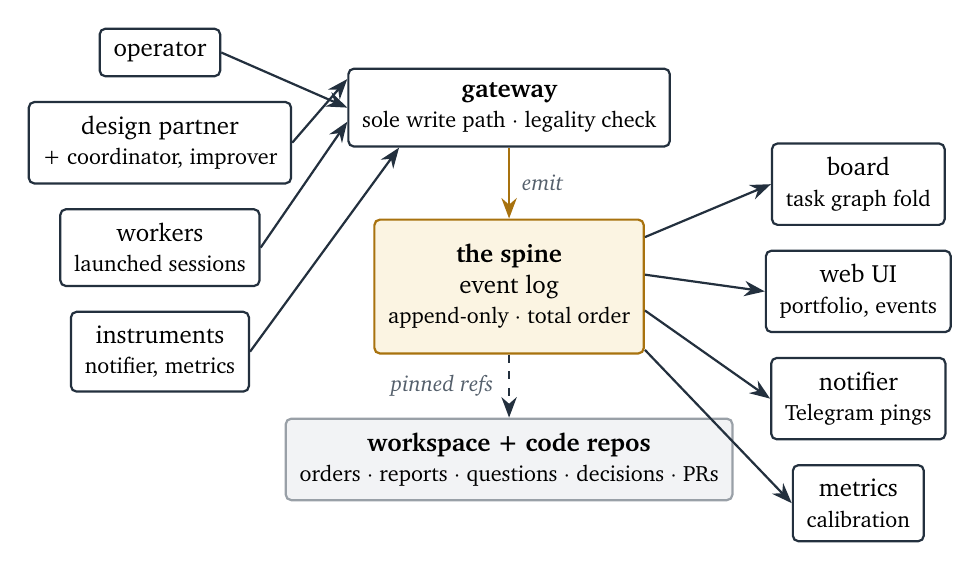
\begin{tikzpicture}[node distance=6mm]
  % spine
  \node[hboxaccent, minimum width=34mm, minimum height=17mm] (spine) {\textbf{the spine}\\event log\\\footnotesize append-only $\cdot$ total order};
  \node[hbox, above=9mm of spine, minimum width=30mm] (gw) {\textbf{gateway}\\\footnotesize sole write path $\cdot$ legality check};
  % actors (left)
  \node[hbox, left=16mm of gw, yshift=7mm] (op) {operator};
  \node[hbox, below=3mm of op] (dp) {design partner\\\footnotesize + coordinator, improver};
  \node[hbox, below=3mm of dp] (wk) {workers\\\footnotesize launched sessions};
  \node[hbox, below=3mm of wk] (inst) {instruments\\\footnotesize notifier, metrics};
  % projections (right)
  \node[hbox, right=16mm of spine, yshift=13mm] (board) {board\\\footnotesize task graph fold};
  \node[hbox, below=3mm of board] (ui) {web UI\\\footnotesize portfolio, events};
  \node[hbox, below=3mm of ui] (tg) {notifier\\\footnotesize Telegram pings};
  \node[hbox, below=3mm of tg] (met) {metrics\\\footnotesize calibration};
  % workspace
  \node[hboxdim, below=8mm of spine, minimum width=42mm] (ws) {\textbf{workspace + code repos}\\\footnotesize orders $\cdot$ reports $\cdot$ questions $\cdot$ decisions $\cdot$ PRs};
  % arrows
  \draw[harrow] (op.east) -- (gw.west);
  \draw[harrow] (dp.east) -- (gw.170);
  \draw[harrow] (wk.east) -- (gw.185);
  \draw[harrow] (inst.east) -- (gw.200);
  \draw[harrowaccent] (gw.south) -- node[hlabel, right=1pt]{emit} (spine.north);
  \draw[harrow] (spine.20) -- (board.west);
  \draw[harrow] (spine.5) -- (ui.west);
  \draw[harrow] (spine.-10) -- (tg.west);
  \draw[harrow] (spine.-25) -- (met.west);
  \draw[harrow, dashed] (spine.south) -- node[hlabel, left=2pt]{pinned refs} (ws.north);
\end{tikzpicture}
\caption{The system in one picture. Every actor writes through one gateway into one log; every surface anyone reads is a deterministic projection of that log; content lives in git, referenced by immutable pins.}
\end{figure}

Everything else in this document is detail on this picture: what the events are, who may emit them, what the projections show, and how a system this simple runs real multi-agent work.

% =========================================================================
\section{Vision and Lineage}
% =========================================================================

\subsection{Ben's OmegaHive1 and 1.1}

OmegaHive1 (June 2026) specified a cooperative hive of OmegaClaw and OpenClaw agents with a dual purpose: real research output, and methodological knowledge about what makes collectives work. Its architecture requirements --- deliberately independent of any particular agent roster --- are the backbone we build against. Four of them shaped us most.

\textbf{Two-tier communications, mechanically curated.} Fast working traffic and human-legible reporting are separate layers, and what gets promoted to humans is decided by rules, not by agents' sense of what is interesting:

\begin{benquote}
Crucially, the fast tier is curated out of Slack, not hidden from humans: every bus message is persisted and inspectable\ldots{} so the distinction between tiers is editorial, not one of visibility. \ldots{} Mechanical promotion rules are preferred over agent self-reporting of what humans would find interesting.
\benattrib{OmegaHive1, \S2.2 (Two-tier communications)}
\end{benquote}

\textbf{Task ownership on a board, not in chat.} All non-trivial work flows through a shared board with explicit ownership, status, and provenance. The 1.1 revision sharpened this to a principle we quote often:

\begin{benquote}
All non-trivial work enters the task graph. Chat alone is not a task-management system.
\benattrib{OmegaHive 1.1, \S3.3 (Task graph)}
\end{benquote}

\textbf{Provenance and editorial discipline.} Documents carry notes-and-sources companions; an editor gates completion on their validity; writers source from the raw record, not from each other's summaries --- serial error propagation through summarization chains is named as the enemy.

\textbf{Governance as mechanism, not prompt.} Permission tiers are enforced ``at the gateway and credential level, not merely in prompts,'' and a human-only recovery path is maintained at all times:

\begin{benquote}
A human-only, out-of-band recovery path (plain SSH with no agent in the loop) is maintained at all times, so that no failure of the self-managing infrastructure, including the sys-admin agent itself, can lock humans out.
\benattrib{OmegaHive1, \S2.8 (Fleet management and recovery)}
\end{benquote}

OmegaHive 1.1 (July 2026) revised the roster model --- ``a small persistent core that owns stable responsibilities, plus a spawn-on-demand layer'' for bounded work --- added an asynchronous task queue with atomic claim, made rejected and expired work first-class evidence rather than embarrassment, added a runtime safety floor and a Tier~1.5 (act only through adjudication), and set the bar in one sentence:

\begin{benquote}
Every non-trivial task has an owner, contract, audit trail, budget, evidence trail, and completion criterion.
\benattrib{OmegaHive 1.1, Abstract}
\end{benquote}

\subsection{Our derivation: three moves}

We derived our design from these requirements with three moves, each a simplification the specs permit but do not demand.

\textbf{One log instead of three stores.} The specs describe a bus, a board, and a queue. We collapsed them: one event log, with the board and the queue as folds over it. Independent stores drift, and reconciliation code is where correctness goes to die; a projection cannot disagree with its source. The two-tier communication requirement survives fully --- the fast tier is the log itself, and the human tier is a mechanically-promoted rendering of it. We derive the channel from the ledger.

\textbf{One gateway, one policy.} Whatever writes, writes through a single gated emit whose legality rules are one declarative structure shared by the acceptance check and the board fold. Enforcement is structural: a document task cannot \emph{reach} done without a passed review, no matter what any agent says --- the transition is unreachable, not discouraged.

\textbf{Functions before residents.} Every role in the specs --- chief of staff, conscience, librarian, editor --- is real, but none starts as a long-lived process. A role is an authority row plus a rehydration bundle --- the committed state a fresh session reads in order to wake as that role: data, not a daemon. Roles become resident agents one at a time, when the evidence says the function earns a seat. Section~7 shows how far along that path we are.

\subsection{The empirical detour that set the course}

Before running real work we ran a coordinator experiment: a funded grid comparing LLM coordinators (strong and cheap models, with and without curated knowledge) against a mechanical greedy policy, each coordinating scripted workers over synthetic task boards --- dependency graphs with joins and scheduled failures, completion scored against a fixed time and call budget. The result was humbling in a useful direction. The mechanical policy completed 20 of 20 seeds at zero cost, because every generated board's single join was already satisfied by one of its branches: the optimal policy was inaction, and the do-nothing policy is free. The LLM cells burned their budgets --- the cheap tier mostly on output the command parser rejected --- and a sensitivity probe that tripled the strong model's wall-clock held completion flat while decisions, prunes, and waste all rose. Not latency, not budget: action bias. The honest verdict: we had not yet posed a question that discriminates coordination quality, and a synthetic coordination environment is valid only if the null policies provably fail it --- a rule we now pre-register for any future attempt. The grid licenses nothing as a comparison; what survives is three narrower findings --- over-intervention is the LLM-coordinator failure mode, below a capability bar the interface dominates cognition, and boards must be validated against null policies before use --- and they are all we carry forward.

Two consequences shaped everything since. \emph{Coordination is not the binding constraint until the spine proves otherwise}: the real hive runs a mechanical coordination core, the LLM consulted only at defined trigger points, and we stopped iterating synthetic experiments --- real coordination episodes accumulate in the log and become replayable test cases when they arrive. And \emph{the hive's first workload is the hive}: four days of running the project as a pseudo-hive --- work orders drafted in chat, a human copy-pasting questions and answers between sessions --- had shown exactly where coordination actually hurts --- questions and answers with no durable home, plan state living in one person's memory, knowledge dying in transcripts. So the substrate of record went live and the hive started building itself through it. Every mechanism in the next two sections was delivered as a work order through the loop it describes.
        % 1 introduction · 2 one page · 3 vision and lineage
% =========================================================================
\section{Key Concepts}
% =========================================================================

\subsection{The spine: events, runs, time}

An event is a small record: an actor, a role, a type, a task id where relevant, and a payload of references and short structured fields. \code{task.created}, \code{task.assigned}, \code{task.blocked}, \code{task.reported}, \code{review.passed}, \code{gateway.rejected} --- coordination facts, never content. Events live in Postgres, append-only, in \emph{runs}: one run per project, each run a bounded, totally-ordered span with its own board. Time is server-set --- a per-run monotonic logical timestamp assigned under the emit lock --- so no client clock is ever trusted and every duration in our metrics is a difference of positions in the record, not of laptops' opinions.

Two mechanisms make the log safe for concurrent, fallible, out-of-process writers. \emph{Idempotency}: every emit carries a content-derived key --- a hash of the run, actor, operation, payload, and the log position the writer had observed --- so two emits share a key exactly when they are the same decision made from the same observed board, and retries never duplicate. \emph{Generation tokens}: every read carries a token that a restore-from-backup bumps, so a client holding a cursor from before the restore gets a refusal, drops its cursor, and re-reads --- a restore can never silently strand a live reader on a phantom history.

\subsection{Legality: one specification, checked on the way in}

Who may emit what, from which task state, is one declarative table. The gateway evaluates it before appending; the board fold applies the same table when projecting. One specification, two consumers --- so the failure class ``accepted but silently changes nothing'' is gone by construction. A worker emitting \code{task.accepted} on a task assigned to someone else is refused with \code{ALREADY\_OWNED}; the refusal is itself an event, visible in every projection. Refusals are diagnostic data, not embarrassment --- when a wave of them appears, something upstream is misconfigured, and the log says exactly what.

The task lifecycle the legality table governs:

\begin{figure}[h]
\centering
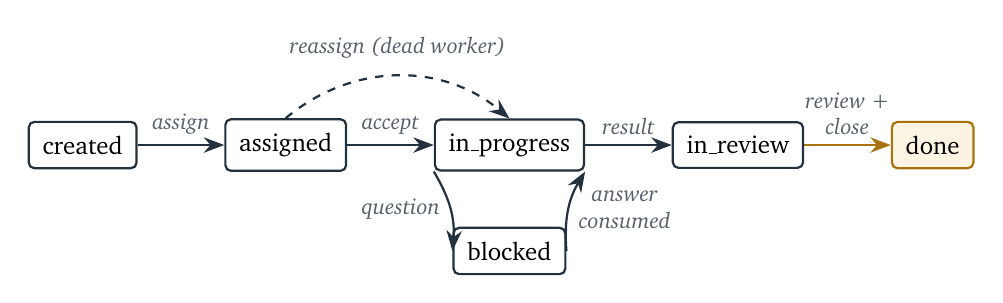
\begin{tikzpicture}[node distance=9mm and 11mm]
  \node[hbox] (created) {created};
  \node[hbox, right=of created] (assigned) {assigned};
  \node[hbox, right=of assigned] (prog) {in\_progress};
  \node[hbox, below=7mm of prog] (blocked) {blocked};
  \node[hbox, right=of prog] (review) {in\_review};
  \node[hboxaccent, right=of review] (done) {done};
  \draw[harrow] (created) -- node[hlabel, above]{assign} (assigned);
  \draw[harrow] (assigned) -- node[hlabel, above]{accept} (prog);
  \draw[harrow] (prog) -- node[hlabel, above]{result} (review);
  \draw[harrowaccent] (review) -- node[hlabel, above]{review +\\close} (done);
  \draw[harrow, bend left=18] (prog.south west) to node[hlabel, left]{question} (blocked.west);
  \draw[harrow, bend left=18] (blocked.east) to node[hlabel, right]{answer\\consumed} (prog.south east);
  \draw[harrow, dashed, bend left=40] (assigned.north) to node[hlabel, above=1mm]{reassign (dead worker)} (prog.north);
\end{tikzpicture}
\caption{Task lifecycle. Worker-owned transitions (accept, block, unblock, result) and operator-owned ones (assign, review, close) are separated by the legality table, not by convention. \code{done} is unreachable without a review event.}
\end{figure}

\subsection{Refs, not bulk: the workspace}

The log carries references; content lives in git. The \emph{workspace} repository is the project's paper trail, one directory per project: \code{orders/} (one file per task --- the task's contract), \code{reports/} (worker results), \code{questions/} (blocking questions as files), \code{decisions.md} (append-only decision log), plus the project charter, roadmap, and operating docs. The \emph{code repo} holds the software and takes changes only as pull requests.

The join between log and git is the pin: every reference emitted into the spine is \code{path@sha}, minted only after the content is committed and pushed. Tooling refuses to mint a pin for uncommitted content. The consequence is a strong property bought cheaply: an unprovenanced claim is structurally impossible. A result event points at an exact immutable version of a report; a review event points at the result it certifies; replaying the log years later resolves every citation to the byte.

\subsection{Roles, identity, and the honest caveat}

Four roles today: \emph{human} (the operator and the seat functions acting with human-tier authority), \emph{coordinator} (assignment and plan mutation), \emph{worker} (one per launched session, registered at launch), and \emph{instrument} (deterministic emitters --- the notifier, the metrics generator --- which never judge anything). A launched worker's only write path is a wrapper script issued at launch with its run, role, and actor id baked in --- a proto-credential the worker cannot misstate. Three named functions operate at human tier today --- the \emph{design partner} (authors a project's orders and its defining documents), the \emph{coordinator} (composes waves from the ready order stock), and the \emph{improver} (runs the retros) --- each a role over durable state, woken per \emph{sitting} (one continuous stretch of operator engagement); why they are seats in rehearsal rather than resident agents is Section~7's subject.

The caveat we state plainly: identity is assertion, not mechanism. Any process on the host could claim any role; the audit answers \emph{what was legal}, not \emph{who really}. This is an accepted, recorded posture --- safe while every writer enters through operator-controlled hardware, and exactly the thing the \emph{identity gate} of Section~7 (below, simply: the gate) exists to close before any long-lived agent holds authority.

\subsection{A task's life, in events}

Concretely --- a small real task, as the log records it:

\begin{casebox}
\begin{tabular}{@{}p{40mm}L{88mm}@{}}
\code{worker.registered} & operator registers \code{sess-cli-polish-0721} \\
\code{task.created} & order pinned: \code{orders/cli-polish.md@41c2f9e} \\
\code{task.assigned} & to the registered worker \\
\code{task.accepted} & the session's first act --- refused unless assigned to it \\
\code{task.reported} & \code, ref to a committed question file \\
\code{task.blocked} & \code{needs: decision} --- the worker stops; the operator's phone buzzes \\
\code{task.unblocked} & the answer arrived as a commit to the order; the worker consumed it \\
\code{task.result\_posted} & ref to the pinned result report \\
\code{review.passed} & the operator's judgment, referencing the result it certifies \\
\code{task.status\_override} & \code{done} --- reachable only past the review \\
\end{tabular}
\end{casebox}

Ten events, four pinned documents, and no self-report load-bearing anywhere: every step is either a recorded judgment or a refusal waiting to happen.

% =========================================================================
\section{The Hive Today}
% =========================================================================

\subsection{The operator's day}

The interface in one line: \emph{Telegram pushes, the UI shows, SSH writes.} A task costs the operator four judgments, each about one command's worth of clerical residue:

\textbf{Launch.} \code{hive-launch <order-file>} seeds the task on the board with its order pinned, registers and assigns a worker, provisions its private git clones of the workspace and code repos, issues the wrapper, opens a tmux window named after the task, and pastes the kickoff. The worker starts unattended --- autonomous permissions are the launch default, bounded by the wrapper-only write path, per-worker file scoping, and command deny rules, with the pane watchable throughout; the fuller answer is the gate's OS-separation step. One judgment: the order is ready.

\textbf{Answer.} The phone buzzes --- who, what, topic, with a deep link into the board. \code{hive-answer <task> "<text>"} appends the answer to the order's Answers section, commits, pushes, and nudges the worker's pane itself. One judgment. Append-only by design: amendments flow as commits to the order, and the worker re-reads its order at HEAD before acting --- the latest committed order supersedes its memory of it.

\textbf{Merge.} The pull request, reviewed in the ordinary way --- deliberately outside the hive. This is the engineering judgment on the artifact, and it stays on engineering's home turf.

\textbf{Close.} \code{hive-close <task>} verifies the board state, pulls the result ref from the spine's own record, emits the review verdict and the close --- then scores the task's predictions and commits the updated metrics, automatically. One judgment: the result holds.

A launch refuses when too many tasks sit in review --- the throttle counts \code{in\_review} across every project, because the limit is the operator's review bandwidth, not any project's. When that refusal fires regularly, review is the bottleneck; the correct response is to slow down or deepen review, and the system makes the signal impossible to miss. Daily, one heartbeat message summarizes every run; silence one hour past its scheduled time is itself the alarm.

\begin{figure}[h]
\centering
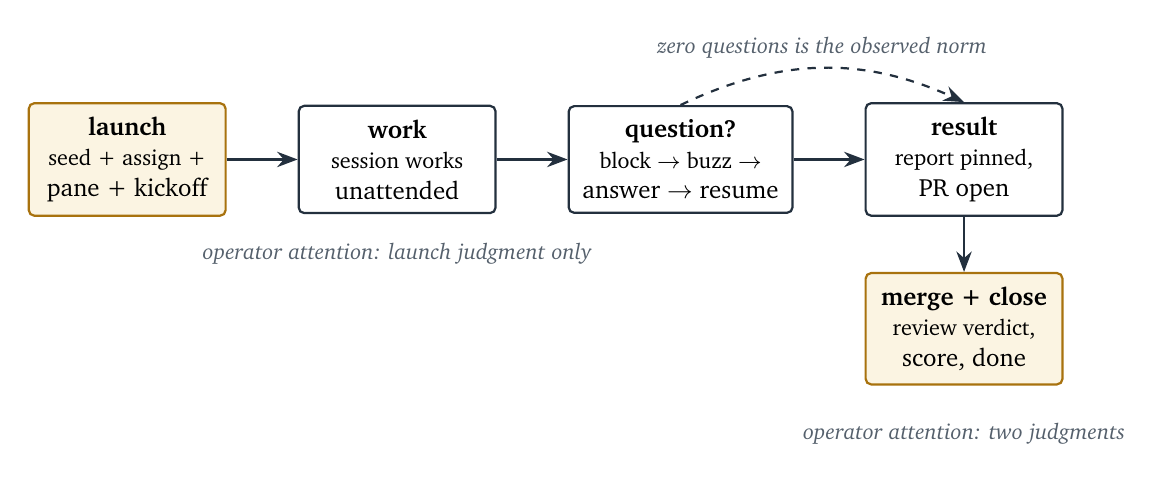
\begin{tikzpicture}[node distance=7mm and 9mm]
  \node[hboxaccent, minimum width=25mm] (launch) {\textbf{launch}\\\footnotesize seed + assign +\\pane + kickoff};
  \node[hbox, right=of launch, minimum width=25mm] (work) {\textbf{work}\\\footnotesize session works\\unattended};
  \node[hbox, right=of work, minimum width=25mm] (qa) {\textbf{question?}\\\footnotesize block $\to$ buzz $\to$\\answer $\to$ resume};
  \node[hbox, right=of qa, minimum width=25mm] (result) {\textbf{result}\\\footnotesize report pinned,\\PR open};
  \node[hboxaccent, below=of result, minimum width=25mm] (close) {\textbf{merge + close}\\\footnotesize review verdict,\\score, done};
  \draw[harrow] (launch) -- (work);
  \draw[harrow] (work) -- (qa);
  \draw[harrow] (qa) -- (result);
  \draw[harrow] (result) -- (close);
  \draw[harrow, dashed, bend left=25] (qa.north) to node[hlabel, above]{zero questions is the observed norm} (result.north);
  \node[hlabel, below=2.5mm of work] {operator attention: launch judgment only};
  \node[hlabel, below=2.5mm of close, yshift=-1mm] {operator attention: two judgments};
\end{tikzpicture}
\caption{The Phase 1 loop. Four operator judgments per task; everything between them runs on the spine.}
\end{figure}

\subsection{Workers: sessions, not services}

Our workers are launched CLI coding-agent sessions (Claude Code today; the binding is tool-agnostic). The participation contract is short: operate as your registered actor; stay inside your order's scope and stop-lines; speak only through the spine; put content in the workspace and emit pinned refs; when your order under-determines something with frozen consequences, \emph{do not extrapolate --- ask}, by writing a question file, blocking, and stopping; consume answers from the order at HEAD, never from chat; externalize your state before every stop.

Silent extrapolation is the defect; the interruption is the feature. And blocking is free: an idle session at its prompt makes zero API calls, and in headless mode the process simply exits between turns --- a blocked worker is state, not a process. This inverts the economics of Ben's resident-agent picture in a way we consider load-bearing: a continuous agent loop pays tokens to keep \emph{being}, and free-running is also precisely the over-intervention failure our coordinator experiments punished. Session workers are natively trigger-driven. Waiting costs nothing; acting requires a reason.

Worker death is a normal event, not an incident. A session that dies or degrades is replaced, never resurrected: a fresh worker id, a reassignment on the record, a kickoff citing the last pinned report --- the new session starts from externalized state. Nothing that matters lives in a process.

\subsection{The instruments}

Deterministic emitters, no judgment anywhere in them. The \emph{notifier} watches the spine and renders attention events --- questions, blocks, escalations, results --- to Telegram, each with a deep link into the web UI; plus the daily heartbeat. The \emph{metrics generator} projects per-task durations with clock ownership made explicit: operator-clock spans (how long an answer waited) are the hive's own latency and never a worker-performance signal; worker-clock spans are the session's. The hive never grades itself --- numbers come from deterministic folds, verdicts from humans.

The one instrument with teeth at launch time: \emph{predictions}. Every order carries a committed prediction --- expected effort against the project's own recorded medians, expected question count, expected review outcome, named risks --- and the launcher refuses an order without one. At close, the prediction is scored against the spine and appended to a calibration ledger. Predictions are honest guesses, never commitments; calibration is the product, not the number.

\subsection{The web UI and the portfolio}

Server-rendered, tailnet-only today, and structurally boring on purpose: it constructs the same \emph{port} client every process uses --- the one small library that reads the log and emits through the gateway --- and holds no state that is not an event --- kill it, replay the log, and it renders identically. The entry point is the portfolio: every live project's board on one page, active work plus recent closes by default, full history a click away. Per-run views show the board, the raw event stream with refusals styled distinctly, and metrics. A ticker renders events as one-line sentences (``w1 claimed t3'', ``\texttimes\ w2 refused t3: ALREADY\_OWNED'') --- the single feature that makes the thing feel alive, and every line of it a deterministic rendering of the log.

The hive runs multiple projects on one substrate: each is a run with its own board, orders, and reports, its committed identity in a small \code{project.conf}, and its own effort baselines --- work-shapes differ, so calibration is per-project. The hive itself is project number one; the first tenant --- a PLN benchmarking project, real work: re-validating PLN reasoning benchmarks against current Hyperon components --- seeded in a day and launched through the same tools. The portfolio surfaces --- one board, one heartbeat, one notifier across all runs --- exist because operating two projects immediately made per-project surfaces feel like toil. That is the standing pattern: overhead complaints are data, and a step that feels clerical twice gets named as a pain with a proposed fix.

\subsection{What it runs on}

One modest host. A container stack --- Postgres (loopback-only), the hive image (gateway library, CLI, migrations, tests --- one image, many one-shot services), the notifier, the UI --- under rootless Podman with pinned digests. Secrets live per-service in an operator-owned directory, referenced by a committed names-only manifest; nothing secret ever lands in the log or the repos. Backups are drilled, not assumed: a scheduled dump of the log store, a mirrored workspace, and a rehearsed restore whose generation bump makes stale readers refuse rather than silently diverge. Every deployment is pinned --- container images, the patched OmegaClaw fork's commit, the policy hash --- so a deployment can be rebuilt from its lockfile plus its backups. Remote operation is a tailnet carrying plain SSH: transport, not trust, with the human-only recovery path Ben's spec demands preserved exactly (keys-only \code{sshd}, no agent in that loop).

\begin{figure}[h]
\centering
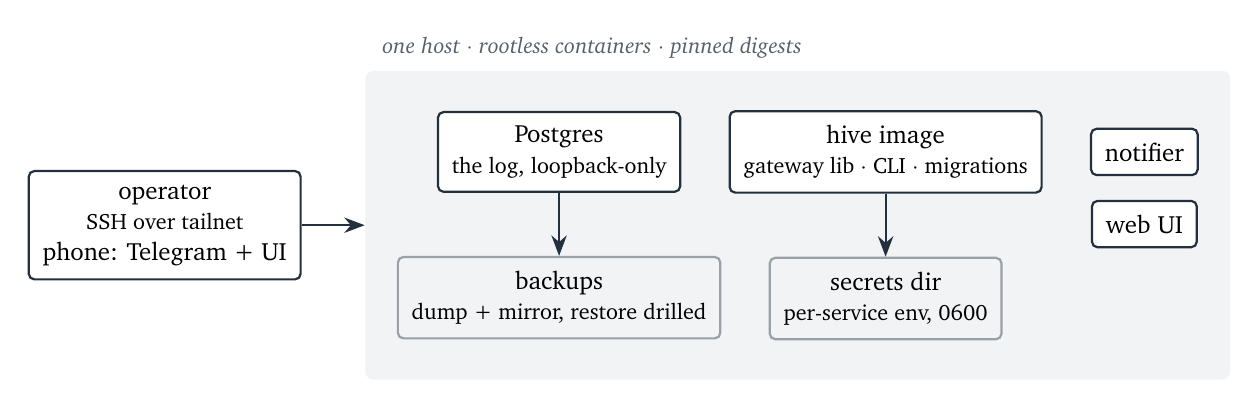
\begin{tikzpicture}[node distance=5mm and 6mm]
  \node[hbox] (pg) {Postgres\\\footnotesize the log, loopback-only};
  \node[hbox, right=of pg] (img) {hive image\\\footnotesize gateway lib $\cdot$ CLI $\cdot$ migrations};
  \node[hbox, right=of img] (not) {notifier};
  \node[hbox, below=3mm of not] (ui) {web UI};
  \node[hboxdim, below=8mm of img] (sec) {secrets dir\\\footnotesize per-service env, 0600};
  \node[hboxdim, below=8mm of pg] (bak) {backups\\\footnotesize dump + mirror, restore drilled};
  \begin{scope}[on background layer]
    \node[fill=palegrey, rounded corners=3pt, inner xsep=4mm, inner ysep=5mm, fit=(pg)(img)(not)(ui)(sec)(bak)] (host) {};
  \end{scope}
  \node[hlabel, anchor=south west] at ($(host.north west)+(1mm,0.3mm)$) {one host $\cdot$ rootless containers $\cdot$ pinned digests};
  \node[hbox, left=8mm of host] (op2) {operator\\\footnotesize SSH over tailnet\\phone: Telegram + UI};
  \draw[harrow] (op2.east) -- (host.west);
  \draw[harrow] (img.south) -- (sec.north);
  \draw[harrow] (pg.south) -- (bak.north);
\end{tikzpicture}
\caption{Deployment. Boring by design: one host, one compose profile, secrets outside the repos, backups that have actually been restored.}
\end{figure}

\subsection{A defect's life: the launch-pane story}

One task, end to end, because it shows the properties this document keeps claiming.

\begin{casebox}
\textbf{Found by use.} July 27, the sitting's third launch: \code{hive-launch} seeds the task, provisions the worker's git clones, issues the wrapper --- then dies opening the tmux window: \code{create window failed: index 4 in use}. The task is stranded half-launched: owned on the board, no session. Manual recovery works; the defect gets an order the same evening, with a committed prediction (1--2 hours, review outcome: clean).

\textbf{The order's mechanism was wrong; its observation was right.} The order blamed index derivation. The worker reproduced the failure experimentally and found the truth one level deeper: \code{tmux new-window -t hive} does not target a session --- tmux resolves the target by \emph{window-name} matching first, so any worker window whose task id starts with ``hive'' shadows the session and donates its occupied index. Intermittently: two matching windows make the match ambiguous and the command works. A passing launch was never evidence the form was safe.

\textbf{The fix, and the fix's own defect.} Append-by-construction targeting (\code{-a -t '=hive:\{end\}'}), name collisions refused, and half-launches made survivable: the failure path now prints and writes the complete manual finish. The tooling drill --- the scripted harness that exercises the whole launch-answer-close loop against a sandbox --- grew from 70 to 92 assertions, all green, four full runs. Then the independent review pass caught what green could not: the change had moved the drill's cleanup trap ahead of its isolation, so an early abort could have killed the operator's live tmux server --- every worker pane on the host. High severity, introduced by the fix, invisible to a test suite that only exercises the code under test, not the harness's own failure path. Dispositioned in a follow-up PR before close.

\textbf{Scored.} Effort ran over the prediction; the review outcome prediction (``clean'') was wrong, and the calibration ledger says so. The reflection that survives: cleanup paths are where small diffs stop being small, and a more powerful cleanup handler is a blast-radius change first, a convenience second.
\end{casebox}

The loop found the defect, ordered the fix, caught the fix's own regression, and recorded a calibration lesson --- all on its own rails, all replayable. This is what ``the hive builds itself'' means in practice.
         % 4 key concepts · 5 the hive today
% =========================================================================
\section{The Improvement Loop}
% =========================================================================

The methodological half of the OmegaHive purpose --- discovering what makes collectives productive --- needs more than intuition accumulating in one operator's head. We made improvement a recorded loop with the same evidence discipline as the work itself.

\textbf{Pains are data.} A step that feels clerical twice gets written into the operating doc's pain list with a proposed fix. Every piece of tooling the hive owns --- the one-command answer path, the launcher, the notifier, the score-at-close automation --- started as a numbered pain, and the pain list records which order retired it.

\textbf{Predictions become calibration.} Every launched order carries committed predictions; every close scores them against the spine. The ledger accumulates per-project --- effort base rates are per-project, because work-shapes differ --- and after one fully-predicted wave we already know things worth knowing: our effort estimates run slightly hot on multi-surface diffs; our question predictions run high (the observed rate is nearly zero --- we read that as orders over-specified for these workers, and the retros watch for the darker reading, silent extrapolation, which numbers this small cannot yet exclude); our review-outcome predictions are the weakest of the three.

\textbf{The improver reads the record, and repairs bind forward.} A dedicated retro function --- woken fresh, no conversational context, inputs strictly the committed record --- scores the closed wave, compares predictions to outcomes, and stages repairs as concrete document edits. Retro~1 produced eight, from prediction-template amendments to a standing rule that a sitting's proposals are committed or explicitly discarded before it ends. The repairs bound the next wave's orders: the loop's output is the loop's next input.

\textbf{The defect ledger.} Four defects found in the hive by the hive, so far:

\begin{center}\small
\begin{tabular}{@{}L{31mm}L{45mm}L{44mm}@{}}
\toprule
\textbf{Defect} & \textbf{How it surfaced} & \textbf{How it resolved} \\
\midrule
Launcher refused the pre-tooling backlog & First real launch attempt against hand-seeded tasks & Adopt mode, ordered and shipped by a worker the same week \\
Board reader broke on wide task ids & First close of a long-named task; predicted in writing in an earlier report's reflection & JSON projection replaced table parsing; regression case pinned \\
tmux targeting collided on window names & Third launch of a sitting; the fix's review then caught a worse defect the fix itself introduced & Append-by-construction targeting; harness blast-radius lesson recorded (\S5.6) \\
Notifier silently watched a wrong run & A week of truthful heartbeats about an empty run; the config default had been warned about, in writing, twelve days earlier & Interim env fix same hour; structural fix ordered: one notifier watching every run, so the drift surface ceases to exist \\
\bottomrule
\end{tabular}
\end{center}

The pattern across all four: found by use or by review, never by luck; the fix arrived as an ordered task through the loop; and where prevention was possible the fix removed the configuration surface rather than guarding it. Where we grade ourselves honestly: the hive is instrumented and governed at its gates, and its self-knowledge is still descriptive, not predictive --- twenty-odd scored tasks is a baseline, not a trend. The trend is what the next retros are for.

% =========================================================================
\section{The Hive at Full Function --- and the Path There}
% =========================================================================

\subsection{The hive, working, a few months out}

Describe the destination as it functions, then earn it. A day in that hive:

The coordinator seat wakes on the wave boundary. It is not a process that survived the night; it is a credential, a memory directory, and a rehydration bundle --- it wakes, reads the committed state, and composes the next wave from the ready order stock against the review throttle. Its authority is real but narrow: it assigns and launches within the throttle, executing wave plans a human committed. It cannot merge, cannot pass review, cannot close. Those transfers never happen.

Design-partner seats --- one per project --- keep the order stock ahead of demand. Each authors orders from its project's committed context, files predictions, and proposes charter and roadmap changes the operator reviews and commits. The improver wakes after every wave close, alone and fresh, and its retros now carry trend claims: calibration curves over dozens of scored tasks per project, repairs whose effect shows up in the next curve.

Workers are unchanged in kind --- launched sessions, spine-speaking, block-honest --- but the contract has descended the instrumentation ladder --- convention, then hooks, then native tools; step 6 below --- so emits fire from hooks and native tools, and report discipline is code, not model memory. Questions land as native tool calls; the notifier's ping carries them to whichever human owns the judgment.

Identity is mechanism now. Every seat holds a per-seat credential, issued at seat creation, revoked at deletion; the gateway derives role and actor from the credential instead of believing flags. An emit-as-coordinator without the credential is not illegal --- it is impossible. The operator's day is judgment at the boundaries: bless the wave cut, answer the questions only a human can, merge, close. Everything clerical about coordination has become substrate.

And there is more than one hive. A colleague's deployment runs the same pinned profile on their own host with their own projects; what travels between deployments is evidence --- calibration ledgers, retro findings, order patterns that worked --- not access. Each hive is sovereign; the discipline is shared.

\subsection{The path from today, in order}

Each step below exists as a named, triggered item in our committed planning docs; none is speculative. What makes this a path rather than a wishlist: every step has a mechanism, an evidence bar, and a reason it cannot be skipped.

\textbf{1. Sole write path.} Today the gateway library is the only writer by convention on a single database role. The step: two database roles --- gateway-writer and read-only --- closing the raw-SQL side door, so ``only the gateway writes'' becomes a property of the database, not of good behavior. Ordered against the design-partner seat now; the first gate bar.

\textbf{2. OS separation.} The stack moves from the operator's account to a dedicated unprivileged hive user --- own namespace, own volumes, own timers. Prepared and rehearsed live (account, rootless runtime, restore rehearsal, replay-identity check); the cutover waits for a calm hour by policy, because access-layer changes are named, never rushed. The second gate bar: agents stop running as the person who can approve things.

\textbf{3. Credential $\to$ identity at the gateway.} Per-seat secrets from which the gateway derives (role, actor). The launch-issued wrapper already has exactly this shape --- the backing swaps from convention to secret with no seat-facing change. The third gate bar, and the gate's open-test in one line: \emph{emit-as-coordinator becomes impossible without the credential, not merely illegal.}

\textbf{4. Review depth before any credential.} The throttle already paces launches to review bandwidth, but review today certifies ``the operator read the result and saw no red flags.'' Before any seat holds authority, the editorial gates get at least a sketch: independent review as a first-class gated step for document-shaped work --- Ben's editor-and-companion-document requirement, landing as legality rows rather than a resident editor. The gate stays shut until this exists; a credentialed coordinator pacing unexamined work would be automation of negligence.

\textbf{5. Seats graduate one at a time.} Rehearsal is the proving ground, and it is already running: coordinator, improver, and design partners operate today with full function and zero authority, every artifact through a human commit-gate. A seat graduates when its rehearsal record says the function works --- the coordinator's bar, for instance: its wave cuts hold up under operator judgment with per-task acts reduced to merge and close, across tenant waves, before it ever holds the launch credential.

\textbf{6. Workers climb the instrumentation ladder.} Convention $\to$ hooks $\to$ native tools backed by the port client, so key derivation, pinning, and emission live inside tools where they are code. Climbs when forgotten-emit frequency says convention is the bottleneck --- treating forgotten emits as the signal, not as agent failure.

\textbf{7. Deployment number one that isn't ours.} The current wave of work strips host assumptions: portable deploy with a bring-up drill on a machine that is not ours, a front-door README an outsider can follow, reference material filed as reference. The first outside deployment turns portability from a claim into a fact, and starts the evidence exchange that makes ``many hives'' mean something.

\begin{figure}[h]
\centering
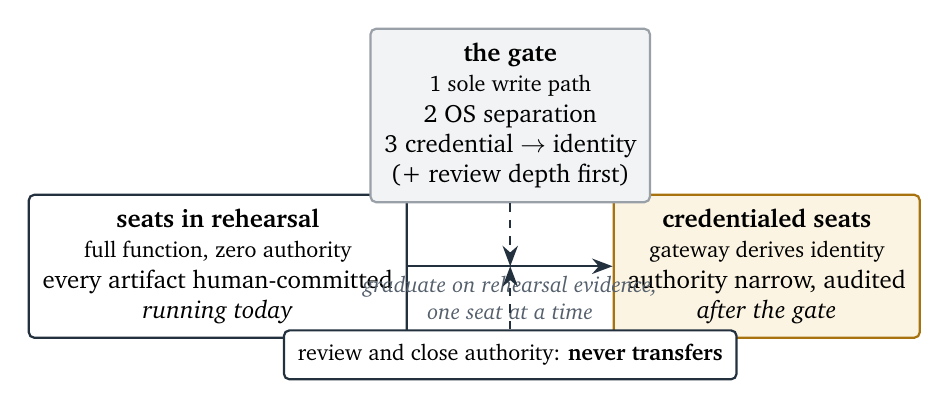
\begin{tikzpicture}[node distance=6mm and 10mm]
  \node[hbox, minimum width=34mm] (rehearsal) {\textbf{seats in rehearsal}\\\footnotesize full function, zero authority\\every artifact human-committed\\\emph{running today}};
  \node[hboxaccent, minimum width=34mm, right=26mm of rehearsal] (cred) {\textbf{credentialed seats}\\\footnotesize gateway derives identity\\authority narrow, audited\\\emph{after the gate}};
  \node[hboxdim, minimum width=23mm, above=8mm of $(rehearsal.east)!0.5!(cred.west)$] (gate) {\textbf{the gate}\\\footnotesize 1 sole write path\\2 OS separation\\3 credential $\to$ identity\\(+ review depth first)};
  \draw[harrow] (rehearsal.east) -- node[hlabel, below]{graduate on rehearsal evidence,\\one seat at a time} (cred.west);
  \draw[harrow, dashed] (gate.south) -- ($(rehearsal.east)!0.5!(cred.west)$);
  \node[hbox, below=8mm of $(rehearsal.east)!0.5!(cred.west)$, minimum width=52mm] (never) {\footnotesize review and close authority: \textbf{never transfers}};
  \draw[harrow, dashed] (never.north) -- ($(rehearsal.east)!0.5!(cred.west)$);
\end{tikzpicture}
\caption{The identity gate. Function is proven in rehearsal before authority exists; authority arrives as a per-seat credential only when all three mechanisms are real; the human judgments at merge and close are permanent.}
\end{figure}

The ordering is the argument. Function before authority, mechanism before trust, evidence before graduation --- the same shape at every step, which is why we believe the path and not just the destination.
   % 6 improvement loop · 7 full function + path
% =========================================================================
\section{Fulfilling the OmegaHive Vision}
% =========================================================================

The claim ``we implement Ben's vision'' should be a table, not a paragraph. Below, each architecture requirement from OmegaHive1 \S2 and the load-bearing 1.1 additions, against the running system --- rows cite their source as (OH1, \S$n$) for OmegaHive1 and (1.1) for the OmegaHive 1.1 revision. \emph{Running} means live today under real work; \emph{rehearsal} means the function operates with a human commit-gate and no authority; \emph{gated} means designed and deliberately blocked on the identity gate; \emph{divergent} means we satisfy the requirement's purpose by a different mechanism, argued afterwards.

\small
\renewcommand{\arraystretch}{1.25}
\begin{longtable}{@{}L{37mm}L{57mm}L{20mm}@{}}
\toprule
\textbf{Requirement (Ben)} & \textbf{Mechanism (running hive)} & \textbf{Status} \\
\multicolumn{3}{@{}l@{}}{\footnotesize\itshape OH1 = OmegaHive1; 1.1 = the OmegaHive 1.1 revision.} \\
\midrule
\endhead
Agent substrate: OmegaClaw + skill-executing agents, LLMs hosted elsewhere (OH1, \S2.1) & Workers are launched CLI coding-agent sessions; OmegaClaw binds through the same port (a small patched fork, built and test-qualified --- no OmegaClaw agent is in the daily loop yet); the host runs only glue and shared services & running (sessions); binding built, unused daily \\
Two-tier communications; fast tier persisted and inspectable; mechanical promotion rules (OH1, \S2.2) & The spine is the fast tier, persisted by construction; the notifier renders attention events to Telegram by rule, never by agent judgment; the UI is the searchable viewer & running \\
Shared knowledge resources, actively curated (OH1, \S2.3) & The workspace: charters, orders, reports, decisions, indexes --- one repo, one map, conventions enforced by protocol docs. Files and git, deliberately: shared Atomspaces arrive with OmegaClaw residents, not before & running; divergent (git, not Atomspace) \\
Task ownership: all non-trivial work on a board with ownership, status, provenance (OH1, \S2.4; 1.1, \S3.3) & Every work item is a board task folded from the log; ownership and status are legality-governed transitions; provenance is the pin discipline & running \\
Provenance and editorial discipline: notes-and-sources companions; an editor gates completion (OH1, \S2.5) & Every claim-bearing artifact enters the record as \code{path@sha}; results carry a structured report; review-before-done is unreachable to skip. The dedicated editorial gate for outward documents: designed, blocked behind the identity gate & running (pins, review); gated (editorial seats) \\
Governance in a version-controlled constitution injected into context (OH1, \S2.6) & Charter, operating manual, worker protocol, seat protocols --- versioned files that \emph{are} each session's context; anything decided in chat lands in them the same sitting & running \\
Reflective conscience monitoring values and dynamics (OH1, \S2.6) & The improver: wakes fresh, reads only the record, scores calibration, stages repairs. Function first, resident later; a values-and-dynamics scope beyond calibration is future seat work & rehearsal \\
Permission tiers enforced at gateway and credential level, not in prompts (OH1, \S2.6) & Legality table at the gateway (running); launch-issued wrapper as proto-credential (running); per-seat credentials from which the gateway derives identity (the gate itself) & running $\to$ gated \\
Evaluation on two independent tracks: deterministic metrics, plus qualitative review that reads them (OH1, \S2.7) & Metrics are deterministic folds with clock ownership labeled; the improver reads them plus the record and writes the retro; disagreement between the tracks is treated as signal & running \\
Fleet from shared images, config-injected; one-command redeploy (OH1, \S2.8) & One pinned image serves library, CLI, migrations, tests; deployments are lockfile-identified; deploy is scripted and checked & running \\
Human-only out-of-band recovery path, always (OH1, \S2.8) & Plain keys-only SSH over the tailnet, no agent in the loop; access-layer changes are named operator acts, never automated & running \\
Small persistent core + spawn-on-demand workers (1.1) & Seats (durable state, ephemeral process) are the persistent core; launched workers are the spawn layer, one per bounded task & running (workers); rehearsal (seats) \\
Async task queue: atomic claim, structured returns, backpressure (1.1) & The board fold over the log: acceptance is atomic and legality-gated, results are structured events, the review throttle is the backpressure & running \\
Rejected / expired / cancelled work is evidence, not embarrassment (1.1, \S4.4) & Refusals are recorded events, styled visibly in the UI, counted in metrics; failed and retired tasks close honestly on the record & running \\
Model and resource governance as a first-class surface (1.1) & Per-session budgets ride the worker CLI's own accounting; model choice is per-launch configuration. A resource-manager function with its own seat: deferred, trigger named (multi-model executor volume) & partial; deferred with trigger \\
Layered memory with active curation (1.1) & The workspace layers (charter / operating docs / decisions / reports) plus per-seat memory directories; a memory-curator seat waits for the volume that earns it & partial; rehearsal \\
Runtime safety floor inherited by every agent (1.1) & Wrapper-only write path, deny rules, containerized stack, secrets manifest with scoped env; OS-level separation is gate bar two & running $\to$ gated \\
Tier 1.5: act only through adjudication (1.1) & Rehearsal mode is exactly this, applied to whole seats: full function, every act through a human commit-gate & running \\
\bottomrule
\end{longtable}
\normalsize

\subsection{Where we deliberately diverge, and why}

\textbf{One log instead of bus + board + queue.} Three stores that must agree are two reconciliation bugs waiting to happen; consistency across stores is the failure mode, not the feature. Ben's requirements for each tier survive as projections of one record. What would change our mind: a working-traffic volume the log's write path cannot carry --- at which point the fast tier shards \emph{below} the spine, with the spine keeping the coordination facts. Nothing today is within orders of magnitude of that.

\textbf{Session workers instead of resident agent containers as the default executor.} Residency pays a continuous token cost to keep being, and free-running was the precise failure our coordinator grid measured. Sessions are trigger-driven, watchable, and free while blocked --- and OmegaClaw keeps its real niches: Ben-ecosystem compatibility, and cheap-model executors where API pricing applies in any wrapper. The substrate is indifferent: both bind through the same port, and a resident executor is a launch-configuration choice, not an architecture change.

\textbf{Telegram + web UI instead of Slack as the human tier.} One operator on a phone needed pushes and deep links, not channels. The promotion-rules requirement is fully honored --- rendering is mechanical, the raw record is always inspectable. The 1.1 revision made the human layer platform-pluggable, which is the posture we built; a Slack surface for a multi-human hive is a renderer, not a redesign.

\textbf{Functions before residents, one at a time.} Ben's roster describes fifteen agents; we run their functions with one operator, launched workers, and three rehearsing seats. This is sequencing, not disagreement: every non-execution agent is unproven until its function has a track record, and rehearsal is how a function earns its seat. The same sequencing covers the shared services: no Lean pool, browser rig, or Atomspace server runs here today --- each arrives as ordered infrastructure with the first project whose work needs it, and the substrate is indifferent to which services surround it. The roster is the destination; the gate is the road.

\textbf{A human trust anchor, for now.} Where the specs place governance in configuration a conscience agent can act on, we place final authority in operator judgments at merge and close --- and the identity gate is the machinery for delegating everything \emph{below} that line safely. Review authority itself never transfers. If a future editorial-gate track record ever argues for moving that line, it will have to argue against a written rule, on the record, which is exactly how we want that conversation to happen.

% =========================================================================
\section{Running One}
% =========================================================================

A deployment is a lockfile: pinned images, pinned fork, policy hash, plus its secrets directory and its backups. The current wave of work makes the claim ``runs on your machine'' literal --- compose-runtime neutrality, a scripted secrets and workspace bootstrap, a front-door README, and the reference material filed where reference material belongs --- with a bring-up drill executed verbatim on a machine that is not ours as the acceptance test.

What we want from colleagues is not admiration but replication. Run one: your host, your projects, your judgment at the gates. The interesting questions --- does the discipline transfer, do the calibration curves look like ours, what does a second operator's pain list contain --- only have answers at $N \geq 2$. We will trade evidence: calibration ledgers, retro findings, order patterns, defect stories. Whatever survives both of us is the architecture.
    % 8 fulfilling the vision · 9 running one
\appendix

% =========================================================================
\section{Glossary}
% =========================================================================

\small
\begin{description}[style=nextline,itemsep=1pt]
\item[spine] The append-only event log; the single source of truth for coordination facts.
\item[run] The log's scoping container: one project's bounded span of operation, with its own board and total order.
\item[event] One coordination fact: actor, role, type, payload of refs and small fields, server-set position.
\item[gateway] The sole write path. Checks legality, assigns time, records refusals, appends atomically.
\item[legality table] One declarative specification of which role may emit which event from which task state; shared by the gateway check and the board fold.
\item[board] The current task graph --- status, owner, dependencies, provenance --- computed by folding the log, never written directly.
\item[projection] Any view derived deterministically from the log: board, UI, notifier renderings, metrics.
\item[fold] How a projection is produced: replay the log through the legality rules and accumulate the view. Nothing folded is stored; it is recomputed.
\item[port] The spine's client interface --- read the log, emit through the gateway --- packaged as the one small library every process uses.
\item[pin / \code{path@sha}] An immutable reference into a git repo, mintable only for committed, pushed content. The join between the log and all bulk content.
\item[workspace] The project paper-trail repository: charters, orders, reports, questions, decision logs, indexes.
\item[order] One task's contract: context, scope, stop-lines, definition of done, committed predictions.
\item[stop-line] An explicit boundary in an order that the worker must not cross, however tempting.
\item[result report] The worker's one-file deliverable record: what shipped, how verified, what the operator must do, and a reflection.
\item[wrapper] The launch-issued emit script with run, role, and actor baked in --- a worker's only write path, and the proto-credential the seat credential will replace.
\item[instrument] A deterministic emitter (notifier, metrics). Never judges.
\item[throttle] The launch-time refusal when too many tasks sit in review, across all projects. Review bandwidth is the system's pace-setter.
\item[predictions / calibration] Committed pre-launch estimates (effort, questions, review outcome, risks), scored at close into an append-only ledger.
\item[wave] A batch of orders composed against the throttle and launched together; the coordinator's unit of work.
\item[sitting] One continuous stretch of operator engagement. Sittings compose, judge, and commit; waves launch.
\item[worker] A launched session working exactly one task under the participation contract.
\item[design partner] The per-project seat function that authors orders and the project's defining documents.
\item[coordinator (seat)] The hive-wide seat function that composes waves from the ready order stock against the throttle.
\item[improver] The seat function that wakes fresh after a wave, scores calibration, and stages repairs.
\item[seat] A durable role: credential (eventually), memory directory, rehydration bundle, wake pattern. The process is never long-lived.
\item[rehydration bundle] The committed state a fresh session reads in order to wake as a seat --- the seat's memory, enumerable and auditable.
\item[rehearsal] A seat operating with full function and zero authority --- every artifact through a human commit-gate --- building the record that argues for its credential.
\item[the gate] The three mechanisms (sole write path, OS separation, credential-derived identity) that must exist before any seat holds authority.
\item[generation token] A marker bumped on restore-from-backup so stale readers refuse and re-read instead of silently diverging.
\item[half-launch] A launch that failed after the board was seeded; survivable by design, with a printed and filed manual finish.
\end{description}
\normalsize

% =========================================================================
\section{Event Reference}
% =========================================================================

\small
\begin{center}
\begin{tabular}{@{}llL{62mm}@{}}
\toprule
\textbf{Event} & \textbf{Emitted by} & \textbf{Meaning} \\
\midrule
\code{worker.registered} & operator & A worker actor id exists; unknown workers are refused \\
\code{task.created} & operator/coordinator & Task seeded, order pinned \\
\code{task.assigned} & coordinator & Ownership granted; owned tasks refuse re-assignment \\
\code{task.reassigned} & coordinator & Dead-worker replacement; old id never reused \\
\code{task.accepted} & worker & The session's first act; legality-checked against assignment \\
\code{task.reported} & worker & Progress / question / finding / result / reflection --- content by pinned ref \\
\code{task.blocked}, \code{task.unblocked} & worker & Honest stop on an under-determined decision; unblock means \emph{answer consumed} \\
\code{task.result\_posted} & worker & Result report pinned; the close reads this ref \\
\code{review.passed} / \code{review.failed} & operator & The human verdict, referencing the result it judges \\
\code{task.status\_override} & operator & Terminal transitions (done, reopened); review-gated \\
\code{task.escalated} & any (legality-scoped) & Attention demanded above the current tier \\
\code{gateway.rejected} & gateway & A refused emit, with machine-readable code and reason \\
\bottomrule
\end{tabular}
\end{center}
\normalsize

% =========================================================================
\section{Sources}
% =========================================================================

\small
\textbf{Ben's specifications} (excerpted throughout): \emph{OmegaHive1 --- An experimental cooperative hive of OmegaClaw and OpenClaw agents}; \emph{OmegaHive 1.1} (July 5, 2026).

\textbf{The running hive's own record}, from which every operational claim in this document derives: the design document and normative spec (one log, one gateway, roles as configuration); the port, deployment, remote-access, and UI specifications; the worker protocol and operator runbook; the operating manual, decision log, wave briefs, retro, and calibration ledger; and the result reports of the twenty-three closed tasks, each pinned in the spine at its close. The repository and workspace are available to SingularityNET colleagues on request --- and after the current wave, buildable from a clean clone.
\normalsize
     % glossary · event reference · sources

\end{document}
